\begin{appchaptercover}{WPA2 Cracking}{app:wifi-cracking}

\section{Introduction}

To crack a WiFi password, we can take advantage Aircrack-ng which is a suite of open-source software used to monitor wireless networks and "break" WEP and WPA keys from Wi-Fi networks. In this appendix, we shall present the required steps in order to perform a successful attack :
\begin{enumerate}
  \item Prepare the \acrshort{nic}
  \item Analyze target WiFi
  \item Capture a 4-way handshake
  \item Crack the password
\end{enumerate}

\lstset{
  language=bash,
  backgroundcolor=\color{lightgray},
  showstringspaces=false,
  basicstyle=\ttfamily\color{black},
  commentstyle=\ttfamily\color{black},
  keywordstyle=\ttfamily\color{blue}
}

\section{\acrshort{nic} preparation}

The first step is to enable the monitor mode of the network card set up. For this we list the network cards available with airmon. As expected, only the PAU06 network card is listed as wlan0. So, we activate the monitor mode with the following command :

\begin{center}
\begin{minipage}{.75\linewidth}
\begin{lstlisting}
root@kali:~# airmon-ng start wlan0
\end{lstlisting}
\end{minipage}
\end{center}

\begin{center}
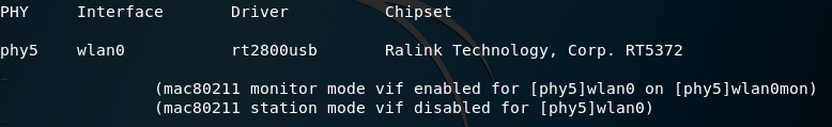
\includegraphics[width=\linewidth]{figures/wpa2-cracking-monitor-mode}
\end{center}

From here, the \texttt{wlan0} network adapter is no longer available, and a new network adapter appears. It can be found by doing an \texttt{ifconfig}. In my case, it is \texttt{wlan0mon}.

\section{WiFi analysis}

Now, we can sniff the network packets circulating around us thanks to airodump. This will allow us to find additional information about the targeted WiFi including the \acrshort{bssid} (the MAC address of the \acrshort{ap}), the CHannel, the AUTHentication mode and the \acrshort{essid} (the name of the \acrshort{ap}).

\begin{center}
\begin{minipage}{.75\linewidth}
\begin{lstlisting}
root@kali:~# airodump-ng wlan0mon
\end{lstlisting}
\end{minipage}
\end{center}

\begin{center}
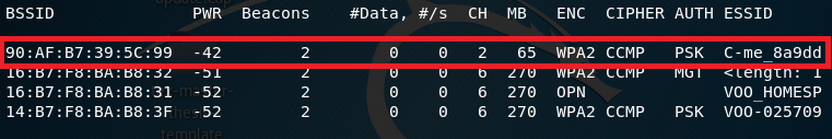
\includegraphics[width=.9\linewidth]{figures/wpa2-cracking-wifi-analysis}
\end{center}

This information will be needed for the next steps.

\section{Handshake capture}

A WPA handshake occurs when connecting a device to the WiFi. Our goal is to capture one to recover the encrypted password. This means that we have to capture the traffic and either wait for a device to connect to the WiFi or induce a disconnection and wait for the device to reconnect. 

To achieve that, we have to start a capture and let it run in the background, still using \texttt{airodump}.

\begin{center}
\begin{minipage}{.75\linewidth}
\begin{lstlisting}
root@kali:~# airodump-ng -c 2 -w capture/ \
	--bssid 90:AF:B7:39:5C:99 wlan0mon
\end{lstlisting}
\end{minipage}
\end{center}

Then in a second console, we have to send deauthentication packets to the desired target.

\begin{center}
\begin{minipage}{.75\linewidth}
\begin{lstlisting}
root@kali:~# aireplay-ng -0 5 \
	-a 90:AF:B7:39:5C:99 -c 24:F0:94:59:DA:B7 wlan0mon
\end{lstlisting}
\end{minipage}
\end{center}

Where :
\begin{itemize}
  \item \texttt{-0} means deauthentication
  \item \texttt{5} is the number of deauths to send; \texttt{0} means send them continuously
  \item \texttt{-a 00:14:6C:7E:40:80} is the MAC address of the access point
  \item \texttt{-c 00:0F:B5:34:30:30} is the MAC address of the client to deauthenticate (that can be found thanks to the previous \texttt{airodump} command already running uner the name station); if this is omitted then all clients are deauthenticated
\end{itemize}

\begin{center}
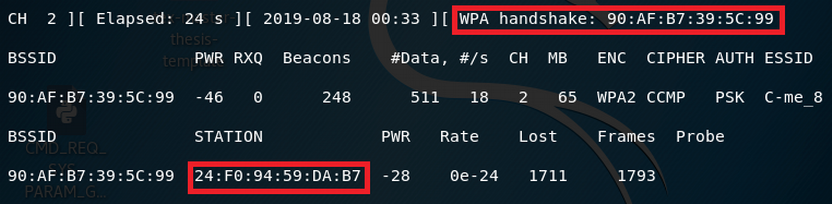
\includegraphics[width=\linewidth]{figures/wpa2-cracking-wpa-handshake}
\end{center}

When successful, an indication with the WPA handshake captured will be displayed the same way as in the figure above. Note that if a device is not set up to automatically reconnect, the deauthentication process may be have succeeded, but we will not get the WPA handshake until the device is connected once again.

\section{Password cracking}

Having a capture containing the handshake, the password is in our hands, inside of the generate .cap file. All is left to do is to crack it, which in this case is possible through either bruteforce or dictionary attack. The bruteforce method is no efficient so we will perform a dictionary attack using the \texttt{RockYou.txt} list discussed in [insert section]. Depending on the speed of your CPU and the size of the dictionary, this could take a long time. To that end, we use \texttt{aircrack-ng} :

\begin{center}
\begin{minipage}{.75\linewidth}
\begin{lstlisting}
root@kali:~# aircrack-ng -w rockyou.txt \
	--bssid 90:AF:B7:39:5C:99 capture-01.cap
\end{lstlisting}
\end{minipage}
\end{center}

Where :
\begin{itemize}
  \item \texttt{-w password.lst} is the name of the dictionary file
  \item \texttt{*.cap} is name of group of files containing the captured packets
\end{itemize}

If a match is found, the WiFi password will be displayed as can be shown in the following figure.

\begin{center}
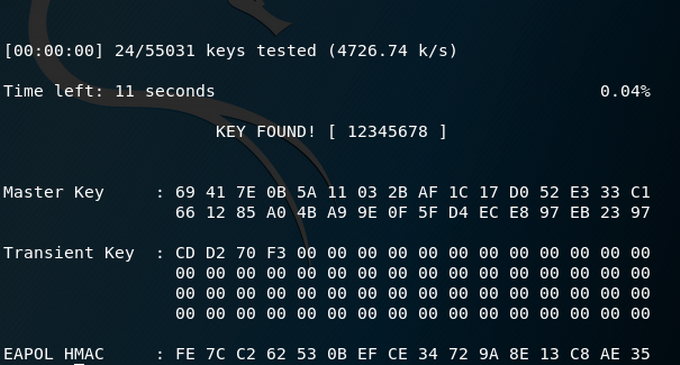
\includegraphics[width=.8\linewidth]{figures/wpa2-cracking-aircrack-ng}
\end{center}

A more in-depth tutorial can be found on the Aircrack-ng official website. \cite{aircrack-ng-wpa-cracking}

\end{appchaptercover}
